% Options for packages loaded elsewhere
\PassOptionsToPackage{unicode}{hyperref}
\PassOptionsToPackage{hyphens}{url}
\PassOptionsToPackage{dvipsnames,svgnames,x11names}{xcolor}
%
\documentclass[
  letterpaper,
  DIV=11,
  numbers=noendperiod]{scrartcl}

\usepackage{amsmath,amssymb}
\usepackage{iftex}
\ifPDFTeX
  \usepackage[T1]{fontenc}
  \usepackage[utf8]{inputenc}
  \usepackage{textcomp} % provide euro and other symbols
\else % if luatex or xetex
  \usepackage{unicode-math}
  \defaultfontfeatures{Scale=MatchLowercase}
  \defaultfontfeatures[\rmfamily]{Ligatures=TeX,Scale=1}
\fi
\usepackage{lmodern}
\ifPDFTeX\else  
    % xetex/luatex font selection
\fi
% Use upquote if available, for straight quotes in verbatim environments
\IfFileExists{upquote.sty}{\usepackage{upquote}}{}
\IfFileExists{microtype.sty}{% use microtype if available
  \usepackage[]{microtype}
  \UseMicrotypeSet[protrusion]{basicmath} % disable protrusion for tt fonts
}{}
\makeatletter
\@ifundefined{KOMAClassName}{% if non-KOMA class
  \IfFileExists{parskip.sty}{%
    \usepackage{parskip}
  }{% else
    \setlength{\parindent}{0pt}
    \setlength{\parskip}{6pt plus 2pt minus 1pt}}
}{% if KOMA class
  \KOMAoptions{parskip=half}}
\makeatother
\usepackage{xcolor}
\setlength{\emergencystretch}{3em} % prevent overfull lines
\setcounter{secnumdepth}{5}
% Make \paragraph and \subparagraph free-standing
\makeatletter
\ifx\paragraph\undefined\else
  \let\oldparagraph\paragraph
  \renewcommand{\paragraph}{
    \@ifstar
      \xxxParagraphStar
      \xxxParagraphNoStar
  }
  \newcommand{\xxxParagraphStar}[1]{\oldparagraph*{#1}\mbox{}}
  \newcommand{\xxxParagraphNoStar}[1]{\oldparagraph{#1}\mbox{}}
\fi
\ifx\subparagraph\undefined\else
  \let\oldsubparagraph\subparagraph
  \renewcommand{\subparagraph}{
    \@ifstar
      \xxxSubParagraphStar
      \xxxSubParagraphNoStar
  }
  \newcommand{\xxxSubParagraphStar}[1]{\oldsubparagraph*{#1}\mbox{}}
  \newcommand{\xxxSubParagraphNoStar}[1]{\oldsubparagraph{#1}\mbox{}}
\fi
\makeatother


\providecommand{\tightlist}{%
  \setlength{\itemsep}{0pt}\setlength{\parskip}{0pt}}\usepackage{longtable,booktabs,array}
\usepackage{calc} % for calculating minipage widths
% Correct order of tables after \paragraph or \subparagraph
\usepackage{etoolbox}
\makeatletter
\patchcmd\longtable{\par}{\if@noskipsec\mbox{}\fi\par}{}{}
\makeatother
% Allow footnotes in longtable head/foot
\IfFileExists{footnotehyper.sty}{\usepackage{footnotehyper}}{\usepackage{footnote}}
\makesavenoteenv{longtable}
\usepackage{graphicx}
\makeatletter
\newsavebox\pandoc@box
\newcommand*\pandocbounded[1]{% scales image to fit in text height/width
  \sbox\pandoc@box{#1}%
  \Gscale@div\@tempa{\textheight}{\dimexpr\ht\pandoc@box+\dp\pandoc@box\relax}%
  \Gscale@div\@tempb{\linewidth}{\wd\pandoc@box}%
  \ifdim\@tempb\p@<\@tempa\p@\let\@tempa\@tempb\fi% select the smaller of both
  \ifdim\@tempa\p@<\p@\scalebox{\@tempa}{\usebox\pandoc@box}%
  \else\usebox{\pandoc@box}%
  \fi%
}
% Set default figure placement to htbp
\def\fps@figure{htbp}
\makeatother

\usepackage{booktabs}
\usepackage{longtable}
\usepackage{array}
\usepackage{multirow}
\usepackage{wrapfig}
\usepackage{float}
\usepackage{colortbl}
\usepackage{pdflscape}
\usepackage{tabu}
\usepackage{threeparttable}
\usepackage{threeparttablex}
\usepackage[normalem]{ulem}
\usepackage{makecell}
\usepackage{xcolor}
\usepackage{fvextra}
\DefineVerbatimEnvironment{Highlighting}{Verbatim}{breaklines,commandchars=\\\{\}}
\KOMAoption{captions}{tableheading}
\makeatletter
\@ifpackageloaded{caption}{}{\usepackage{caption}}
\AtBeginDocument{%
\ifdefined\contentsname
  \renewcommand*\contentsname{Table of contents}
\else
  \newcommand\contentsname{Table of contents}
\fi
\ifdefined\listfigurename
  \renewcommand*\listfigurename{List of Figures}
\else
  \newcommand\listfigurename{List of Figures}
\fi
\ifdefined\listtablename
  \renewcommand*\listtablename{List of Tables}
\else
  \newcommand\listtablename{List of Tables}
\fi
\ifdefined\figurename
  \renewcommand*\figurename{Figure}
\else
  \newcommand\figurename{Figure}
\fi
\ifdefined\tablename
  \renewcommand*\tablename{Table}
\else
  \newcommand\tablename{Table}
\fi
}
\@ifpackageloaded{float}{}{\usepackage{float}}
\floatstyle{ruled}
\@ifundefined{c@chapter}{\newfloat{codelisting}{h}{lop}}{\newfloat{codelisting}{h}{lop}[chapter]}
\floatname{codelisting}{Listing}
\newcommand*\listoflistings{\listof{codelisting}{List of Listings}}
\makeatother
\makeatletter
\makeatother
\makeatletter
\@ifpackageloaded{caption}{}{\usepackage{caption}}
\@ifpackageloaded{subcaption}{}{\usepackage{subcaption}}
\makeatother

\usepackage{bookmark}

\IfFileExists{xurl.sty}{\usepackage{xurl}}{} % add URL line breaks if available
\urlstyle{same} % disable monospaced font for URLs
\hypersetup{
  pdftitle={Curiosity Project: Student Pilot Data Analysis},
  colorlinks=true,
  linkcolor={blue},
  filecolor={Maroon},
  citecolor={Blue},
  urlcolor={Blue},
  pdfcreator={LaTeX via pandoc}}


\title{Curiosity Project: Student Pilot Data Analysis}
\author{}
\date{}

\begin{document}
\maketitle

\RecustomVerbatimEnvironment{verbatim}{Verbatim}{
showspaces = false,
showtabs = false,
breaksymbolleft={},
breaklines
}

\renewcommand*\contentsname{Table of contents}
{
\hypersetup{linkcolor=}
\setcounter{tocdepth}{3}
\tableofcontents
}

The raw data from the student pilot test contained 105 responses. 22 of
the responses were removed because they were missing names and student
ID numbers. An additional 3 responses were removed because they were
either \texttt{Mike} or nonsensical responses to the question asking for
student names (\texttt{Q30\_1}) or student IDs (\texttt{Q30\_2}). The
final sample size is 80 respondents.

\section{Experimental Conditions}\label{experimental-conditions}

The random assignment to conditions appears to have worked fine. The
number of respondents per condition ranged from 18 to 21
(Table~\ref{tbl-expcond}).

\begin{table}

\caption{\label{tbl-expcond}Number of respondents in the control and
experimental conditions.}

\centering{

\begin{tabular}[t]{l|r|r|r|r|r}
\hline
  & Freq & \% Valid & \% Valid Cum. & \% Total & \% Total Cum.\\
\hline
Control & 18 & 22.5 & 22.5 & 22.5 & 22.5\\
\hline
No question, no curiosity prime & 21 & 26.2 & 48.8 & 26.2 & 48.8\\
\hline
Question, no curiosity prime & 21 & 26.2 & 75.0 & 26.2 & 75.0\\
\hline
Question, curiosity prime & 20 & 25.0 & 100.0 & 25.0 & 100.0\\
\hline
Total & 80 & 100.0 & 100.0 & 100.0 & 100.0\\
\hline
\end{tabular}

}

\end{table}%

The manipulation check for the question showed that respondents who were
exposed to a stimulus that contained a question were significantly more
likely to answer ``Yes'' to \texttt{Q24} (``Did the meme you just viewed
contain a question?''; Table~\ref{tbl-mcheck}). Note that the control
condition did not contain a question.

\begin{table}

\caption{\label{tbl-mcheck}Manipulation check for presence of a
question.}

\centering{

\begin{tabular}[t]{l|r|r|r|r}
\hline
  & Control & No question, no curiosity prime & Question, no curiosity prime & Question, curiosity prime\\
\hline
No & 16 & 17 & 6 & 6\\
\hline
Yes & 2 & 4 & 15 & 14\\
\hline
\end{tabular}

}

\end{table}%

\section{Situational Curiosity}\label{situational-curiosity}

Cleaned the items \texttt{Q25\_1} through \texttt{Q25\_4} and determined
the Cronbach's alpha (\(\alpha = .95\)). Did not run a factor analysis
since the correlation matrix showed high significant (\(p < .001\))
inter-item correlations ranging from \(0.74\) to \(0.89\). Combined
items in a mean index (\(M = 3.65\), \(SD = 1.65\)).

There were no significant differences in the mean of situational
curiosity across conditions (Figure~\ref{fig-means}).

\begin{figure}

\centering{

\pandocbounded{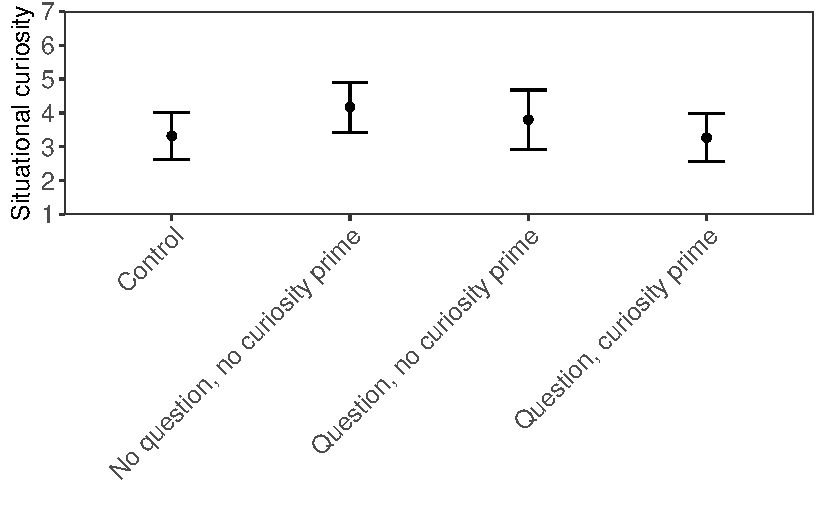
\includegraphics[keepaspectratio]{curiosity_student-pilot_data-analysis_files/figure-pdf/fig-means-1.pdf}}

}

\caption{\label{fig-means}Mean of situational curiosity by experimental
condition.}

\end{figure}%

Examined the cleaned versions of the individual items (\texttt{Q25\_1c}
thru \texttt{Q25\_4c}).

\begin{figure}

\centering{

\pandocbounded{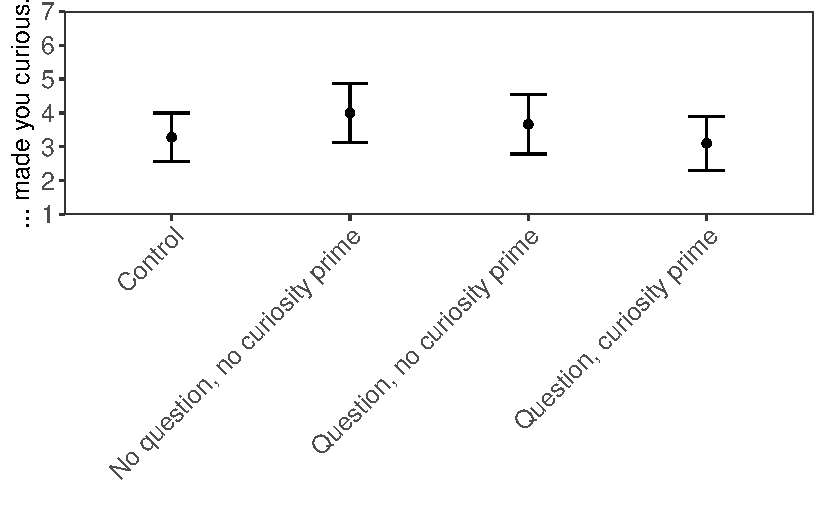
\includegraphics[keepaspectratio]{curiosity_student-pilot_data-analysis_files/figure-pdf/fig-means1-1.pdf}}

}

\caption{\label{fig-means1}Mean of Q25\_1c by experimental condition.}

\end{figure}%

\begin{figure}

\centering{

\pandocbounded{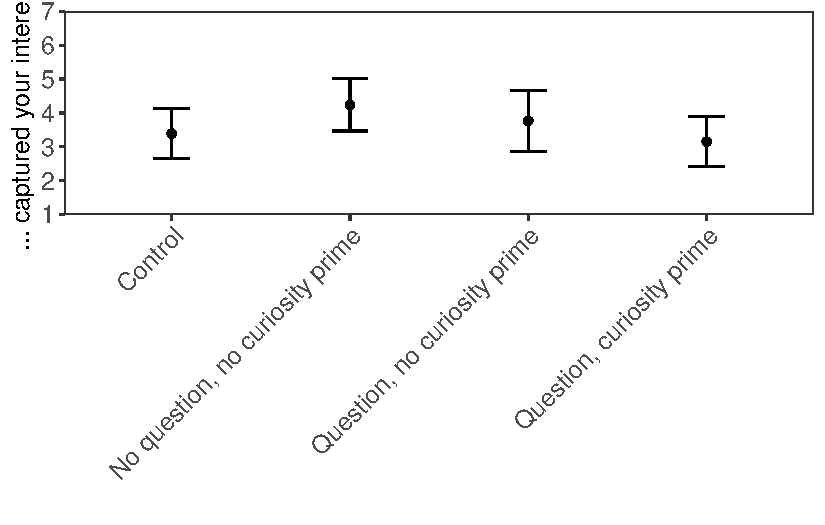
\includegraphics[keepaspectratio]{curiosity_student-pilot_data-analysis_files/figure-pdf/fig-means2-1.pdf}}

}

\caption{\label{fig-means2}Mean of Q25\_2c by experimental condition.}

\end{figure}%

\begin{figure}

\centering{

\pandocbounded{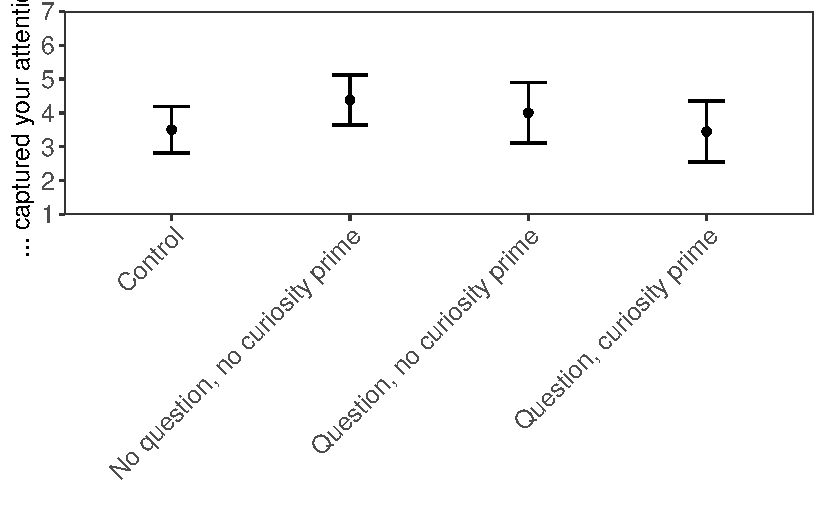
\includegraphics[keepaspectratio]{curiosity_student-pilot_data-analysis_files/figure-pdf/fig-means3-1.pdf}}

}

\caption{\label{fig-means3}Mean of Q25\_3c by experimental condition.}

\end{figure}%

\begin{figure}

\centering{

\pandocbounded{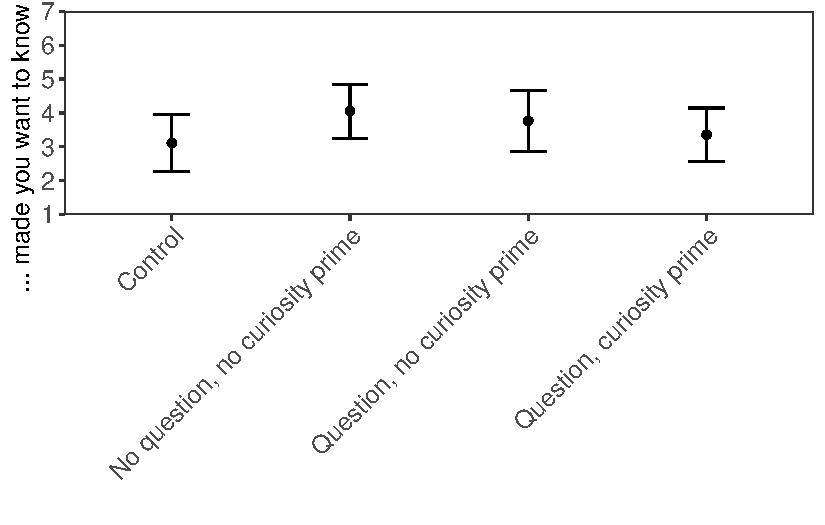
\includegraphics[keepaspectratio]{curiosity_student-pilot_data-analysis_files/figure-pdf/fig-means4-1.pdf}}

}

\caption{\label{fig-means4}Mean of Q25\_4c by experimental condition.}

\end{figure}%




\end{document}
